\documentclass{article}
\usepackage[utf8]{inputenc}
\usepackage{import}
\usepackage[subpreambles=true]{standalone}
\usepackage{graphicx}
\usepackage{amsmath}
\usepackage{amsfonts}
\usepackage{amssymb}
\usepackage{mathrsfs}
\usepackage{enumerate}
\usepackage{fancyhdr}
\usepackage[colorlinks=true,linkcolor=black,anchorcolor=black,citecolor=black,filecolor=black,menucolor=black,runcolor=black,urlcolor=blue]{hyperref}
\usepackage[margin=1.75in]{geometry}
\usepackage{algorithm, algpseudocode}
\usepackage{tikz-qtree}
\usepackage{ulem}
\usepackage{xlop}

\tikzstyle{arr}=[fill=white, draw=black, shape=rectangle, scale=.9]
\tikzstyle{cir}=[fill=white, draw=black, shape=circle, scale=.75]

\begin{document}
%%%%%%%%%%%%%%%%%%%%%%%%%%%%
%%     Chapter Content    %%
%%%%%%%%%%%%%%%%%%%%%%%%%%%%
\section{Integer Arithmetic}
\rule{\textwidth}{1pt}
\subsection{Addition}
As you would expect, the time to add two $n$-digit numbers is proportional to the number
of digits, $\Theta(n)$. Since each digit must be sued to compute the sum.
$$\opadd{1234}{5678}$$
We assume that each digital addition takes constant time (with carry also) and label this
constant $\alpha$. The time to add two $n$-digit numbers is then $\alpha n$.

\subsection{Problem Size}
If we were attempting to determine if a number was prime we would divide it by consectutive primes up
to the quare root of that number. In Computer Science we want to approach all problems in terms of
the problem size. So we should look at both in tmers of the \textit{number of digits} and not
the size of the number. So while the prime identification problem is $\Theta(\sqrt{m})$ where $m$ 
is the number, expressed in binary as $2^n$, $n$ being the number of binary digits results in
$\Theta(2^{n/2})$. Giving an exponential time algorithm.

\subsection{Multiplication}
The elementary approach to multiplication runs in $\Theta(n^2)$ time because every digit on top
is multiplied by every digit on the bottom. There are $2n(n-1)$ atomic additions in this
elementary approach.
$$\opmul{1234}{5678}$$
\subsubsection*{Recursive Multiplication}
By memorizing numbers in large bases, say base 100, $2$-digit decimal numbers can be treated as
$1$-digit numbers in base 100. That makes the multiplication easier, because there will be fewer steps.
To generalize this for $n$-digit numbers, treat them as base $10^{n/2}$ and cut each in half. Each has
$n/2$ digits, and we know the base. Then, recurse through this method until we reach a base we
have memorized. Then multiply them as two $2$-digit numbers, and pull the answer.\\\\
Say we want to multiply two $2$-digit numbers, $ab$ and $cd$, we can then do the following.
$$ad\times bc = ac + (ad + bc) + bd$$
In the example above $ac$ is an $n$-digit number as are $ad$, $bc$, and $bd$.
When adding, $bc$ is not shifted, $bc$ and $ad$ are shifted by $n/2$ digits, and $ac$
is shifted by $n$ digits. Since $ac$ and $bd$ have no overlap you can add them through
concatenation. Then, $ad+bc$ takes $\alpha n$ time and $ac+bd$ is also $\alpha n$ time.
This results in a total add time of $2\alpha n$. \\\\
So without writing out a formal algorithm,
$$M(n) = 4M\left(\frac{n}{2}\right) + 2\alpha n$$
is the recursion we wish to work on. Now, to solve we assume that the base case time
to multiply is $\mu$. The base case is when both of our numbers are $1$ digit long, i.e.
$M(1) =\mu$.

\begin{figure}[H]
\centering
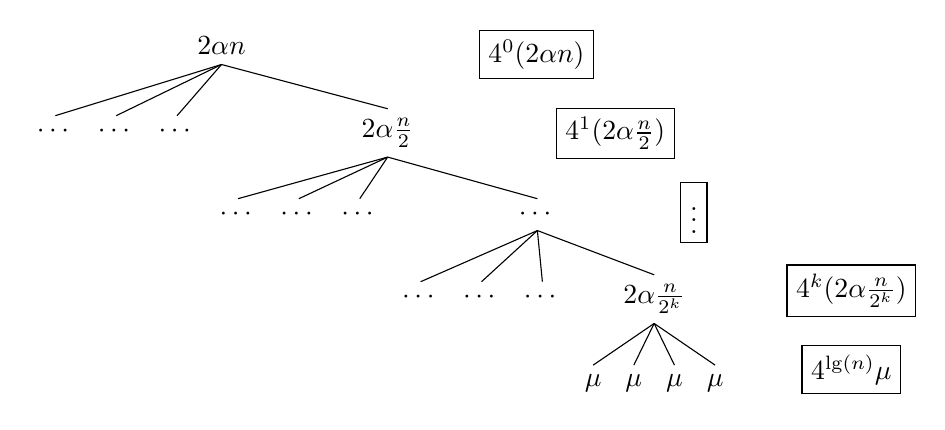
\begin{tikzpicture}
    \Tree [.$2\alpha n$ $\cdots$ $\cdots$ $\cdots$ [.$2\alpha\frac{n}{2}$ $\cdots$ $\cdots$ $\cdots$
        [.$\cdots$ $\cdots$ $\cdots$ $\cdots$ [.$2\alpha\frac{n}{2^k}$ $\mu$ $\mu$ $\mu$ $\mu$ ]]]]
        \node[draw] at (4,0) {$4^0(2\alpha n)$};
        \node[draw] at (5,-1) {$4^1(2\alpha \frac{n}{2})$};
        \node[draw] at (6,-2) {$\vdots$};
        \node[draw] at (8,-3) {$4^{k}(2\alpha \frac{n}{2^{k}})$};
        \node[draw] at (8,-4) {$4^{{\lg(n)}}\mu$};
\end{tikzpicture}
\end{figure}

\noindent Now to calculate the total number of atomic actions,
\begin{align*}
    &= \sum_{i=0}^{\lg(n)-1} (4^i (2\alpha\frac{n}{2^i}) ) + 4^{\lg(n)}\mu \\
    &=2\alpha n \sum_{i=0}^{\lg n-1}\frac{4^i}{2^i} \cdots \\
    &=2\alpha n \sum_{i=0}^{\lg n-1}{2^i} \cdots \\
    &=2\alpha n \left( 2^{\lg n -1 +1} -1 \right) \\
    &=2\alpha n \left( n-1 \right) + 4^{\lg(n)}\mu \\
    &=2\alpha n \left( n-1 \right) + n^{\lg(4)}\mu \\
    &=2\alpha n \left( n-1 \right) + n^{2}\mu \\
    &=2\alpha n \left( n-1 \right)+n^2 \mu
\end{align*}
So we see that with this method we are doing $n^2$ multiplications and $n^2$
additions. In other words, this recursive method has the exact same running time as the
elementary method.

\subsubsection*{Faster Multiplication}

\end{document}